	\documentclass[a4paper, 11pt,oneside,openany, danish]{memoir} % Starter dokumentet af klassen memoir


%%%%%%%%%%%%%%%%%%%%%%%
		       % PREAMBLE %			
%%%%%%%%%%%%%%%%%%%%%%%

% Papirstørrelse og margener
\usepackage[paper=a4paper, hmargin=1.5in, vmargin=0.9in]{geometry}

% Font encoding og sprog
\usepackage[T1]{fontenc}					% Output encoding
\usepackage[utf8]{inputenc}				% Input encoding
\usepackage[danish]{babel}				% Sprog (orddeling)
\renewcommand{\danishhyphenmins}{22} 	% bedre orddeling, minimum to tegn før og efter deling
\usepackage{lmodern}  					% gør underscores pænere
\usepackage{microtype} 					% laver micro ændringer i text for at udgå luft og orddeling

%% Forside text
%\usepackage{soul} % lege lege
%\sodef\an{}{0.2em}{.9em plus.6em}{1em plus.1em minus.1em}
%\newcommand\stext[1]{\an{\scshape#1}}

% Fyldetekst (Lorem ipsum)
\usepackage{blindtext}

% Biblatex til referencer
\usepackage[backend=bibtex]{biblatex}
\addbibresource{bibfil.bib}

% Tabeller
\usepackage{booktabs}
\usepackage{threeparttable}
\usepackage[tableposition=top]{caption}
\usepackage{tabularx}

%matematik
\usepackage{amsmath,amssymb,mathtools,bm}
\newcommand{\tsub}[1]{_{\textup{#1}}}
\def\doubleunderline#1{\underline{\underline{#1}}}
\usepackage[separate-uncertainty = true,multi-part-units=single]{siunitx}

% XColor: Farver
\usepackage[svgnames,dvipsnames,x11names]{xcolor}

% Figurer og floats
\usepackage[]{graphicx}
\graphicspath{{figurer/}}
\usepackage{placeins}
\usepackage{float}			% Muliggoer eksakt placering af floats, f.eks. \begin{figure}[H]

%%% Tegning af kasser
%\usepackage{calc,graphicx,color}
%\definecolor{mygreen}{rgb}{0,0.6,0}
%\definecolor{mygray}{rgb}{0.5,0.5,0.5}

% Biblatex til referencer
%\usepackage[backend=biber]{biblatex}
%\addbibresource{bib.bib}

% Hyper ref
\usepackage[ unicode=true, colorlinks=false, linktocpage=true, 
pdfborder={0 0 0}, pdfstartpage=1, pdfstartview=FitV, breaklinks=true,
pdfpagemode=UseNone, pageanchor=true, pdfpagemode=UseOutlines,
plainpages=false, bookmarksnumbered, bookmarksopen=true,
bookmarksopenlevel=1, hypertexnames=true, pdfhighlight=/O, urlcolor=Black,
linkcolor=Black, citecolor=Black]{hyperref}

% Clever ref
\usepackage{cleveref}



\settocdepth{subsection}
\setsecnumdepth{subsection}

% Sidetal
\let\footruleskip\undefined
\usepackage{fancyhdr}
\usepackage{lastpage}
\pagestyle{fancy} 
\fancyhf{} 

\fancyhead[R]{\leftmark}
\fancyfoot[R]{\thepage \hspace{0.008in} af \pageref{LastPage}}

\fancypagestyle{}{
	\renewcommand{\headrulewidth}{0pt}
	\fancyhf{}
	\fancyfoot[R]{\thepage \hspace{0.008in} af \pageref{LastPage}}%
	
}

% Starten på dokumentet
\begin{document}


%%%%%%%%%%%%%%%%%%%%%%%
		       % FORSIDEN %			
%%%%%%%%%%%%%%%%%%%%%%%

% !TEX root = ../prj4projektdokumentation.tex
% SKAL STÅ I TOPPEN AF ALLE FILER FOR AT MASTER-filen KOMPILERES 
\thispagestyle{empty}
{\centering
	{\scshape\LARGE Aarhus Universitet \par}
	\vspace{1cm}
	{\scshape\Large 4. semesterprojekt gruppe 1\par}
	{\scshape\Large Projektdokumentation\par}
	\vspace{1.5cm}
	{\huge\bfseries Spændingsregulator\par}
	\vspace{2cm}
	{\Large
		201509249 - Caroline Møller Sørensen\\
		201611140 - Sophia Amailie Mortensen\\
		201505195 - Dennis Slot Larsen \\
		201505115 - Laurids Givskov Jørgensen\\
		201508333 - Søren Jensen\\
		13114 - Jeppe Hansen\\  }
	\vfill
	Vejleder\par
	Emir Pasic
	
	\vfill
	
	{\large \today\par}
	\par}





\frontmatter

%%%%%%%%%%%%%%%%%%%%%%%
             % RESUME & ABSTRACT %			
% !TEX root = ../prj4projektrapport.tex
% SKAL STÅ I TOPPEN AF ALLE FILER FOR AT MASTER-filen KOMPILERES 

Denne rapport beskriver et 4. semester projekt ved Ingeniørhøjskolen Aarhus Universitet på studieretningen Elektrisk Energiteknologi. Problemstillingen, der arbejdes med, er at udvikle et system, som kan sikre et stabilt spændingsniveau på en distributionslinje med varierende belastning.

Rapporten beskriver en prototype på en spændingsregulator, som kan installeres på en eksisterende distributionslinje. Prototypen indeholder en simulering af en distributionslinje, hvorpå spændingsregulatorens funktionalitet demonstreres. Reguleringen af spændingen foretages med en trintransformer, som skifter trin på baggrund af data fra måleenheder placeret centralt og decentralt på distributionslinjen.

Projektet indeholder programmering af måleenheder på PSoC, styring af trintransformeren på en Siemens PLC og TCP-kommunikation. 
% !TEX root = ../prj4projektrapport.tex
% SKAL STÅ I TOPPEN AF ALLE FILER FOR AT MASTER-filen KOMPILERES 

This report describes a fourth semester project at Aarhus School of Engineering in the field of Electical Engineering. The thesis is devoted to the development of a system that ensure a stable voltage level on a distribution line with varying load.

The report describes a prototype of a voltage regulator, which can be installed on an existing distribution line. The prototype contains a simulation of a distribution line, on which the functionality of the voltage regulator is demonstrated. The voltage regulation is performed with a step transformer that changes step based on data from measurement devices placed centrally and decentrally on the distribution line. 

The project includes programming of measurement devices on PSOC, controlling/regulation of the step transformer on a Siemens PLC and TCP-communication.


%%%%%%%%%%%%%%%%%%%%%%%


%%%%%%%%%%%%%%%%%%%%%%%
         % INDHOLDSFORTEGNELSE %			
% !TEX root = ../prj4projektrapport.tex
% SKAL STÅ I TOPPEN AF ALLE FILER FOR AT MASTER-filen KOMPILERES 
%%%%%%%%%%%%%%%%%%%%%%%

\tableofcontents

%%%%%%%%%%%%%%%%%%%%%%%
                        % KAPITLER %			
% !TEX root =../prj4projektrapport.tex



\textbf{Praktisk information:} I dette projekt deltog seks ingeniørstuderende fra Ingeniørhøjskolen Aarhus Universitet. De studerende er på 4. semester på studieretningen Elektrisk Energiteknologi. Projektgruppens vejleder er Emir Pasic, der løbende har vejledt gruppen. Semesterprojektets afleveringsdato er 29/5-2017 og bedømmelsesdato er 28/6-2017. \\
\textbf{Læsevejledning:} Henvisninger til projektdokumentationen er lavet med fodnoter, der angiver kapitelnummer og navn på det afsnit, der henvises til. Bilagshenvisninger er lavet med mappenavn og bilagsnummer. \\
\textbf{Tak til:} Der skal tilskrives en tak til Michael Rangård, Specialist Planlægning, og Poul Bagger Thomsen, Afdelingsleder Anlæg 20/0,4kV, fra Eniig for hjælp med data og besøg på transformerstation.

% !TEX root = ../prj4projektdokumentation.tex
% SKAL STÅ I TOPPEN AF ALLE FILER FOR AT MASTER-filen KOMPILERES 


\chapter{Termliste}

\begin{table}[htbp]
	\centering
	\begin{tabular}{|l|l|}
		\hline
		\textbf{Term} 	& \textbf{Beskrivelse} \\\hline
		Spændingsregulator	& Samlet system \\\hline
		Trintransformer	& Transformer med variabelt omsætningsforhold \\\hline
		Trinskifter	& Omfatter trintransformer og relækredsløb  \\\hline
		Styringsenhed	& PLC, HMI og Arduino \\\hline
		Centralt	& Ved trinskifter \\\hline
		Decentralt 	& Ved forbrugeren \\\hline
		Måleenhed	& PSoC og tilhørende hardware \\\hline
		
	\end{tabular}
	\caption{Termbeskrivelse}
	\label{tab:termbeskrivelsen}
	
\end{table}
% !TEX root =../prj4projektrapport.tex

Formålet med dette projekt er at løse følgende problemformulering; \textit{Når belastningerne i et distributionssystem ændres, vil spændingsniveauet variere. Det er vigtigt, at spændingsniveauet holdes stabilt. Hvordan sikres dette?}
Udgangspunktet for problemstillingen er det lovmæssige krav, der siger, at spændingsforsyningen hos danske forbrugere altid skal ligge på 230V $\pm$10$\%$ \cite{Sikkerhedsstyrelsen}. Det ønskes at undersøge udfordringerne ved dette samt at komme med et bud på, hvordan denne problemstilling løses bedst muligt, både som elnettet ser ud i dag, men også i fremtiden. 

For at kunne arbejde med problemformuleringen og undersøge dens aktualitet, valgte projektgruppen at tage kontakt til energiselskabet Eniig. Det viste sig, at der på nuværende tidspunkt ikke foretages regulering på lavspændingsnettet, men i stedet på 60/10 kV transformere. Projektgruppen fandt det derfor interessant at undersøge mulighederne for regulering på lavspændingsnettet og eventuelle fordele og fremtidsaspekter ved dette.

I dette projekt vil fokus derfor være på den del af nettet, der går fra distributionstransformer og ud til forbrugere. For at sikre et stabilt spændingsniveau ønskes det at kunne overvåge tilstanden på distributionslinjen, ikke kun ved transformeren, men også ved hver enkelt forbruger. Det samlede system, der fremstilles i projektet betegnes som Spændingsregulator. Med denne ønskes det at lave et proof of concept i forhold til problemformuleringen. På grund af tilgængelighed af komponenter og udstyr vil prototypen for Spændingsregulator blive skaleret ned. 

For at belyse problemstillingen vil der i dette projekt blive lavet en simulering af en distributionslinje samt belastninger, der skal simulere forbrugere på linjen. Projektet vil desuden bestå af en trintransformer, der giver mulighed for at variere spændingsniveauet til linjen og forbrugerne på sekundærsiden af transformeren.

Til justering af spændingsniveauet, er det nødvendigt at kende til de aktuelle værdier for spændingen både centralt ved trintransformeren og decentralt ved forbrugerne. Af denne grund implementeres enheder til måling af spændingen. Det ønskes desuden at kende til systemets power factor, og derfor skal strømmen også måles. Et eventuelt indhold af harmoniske kan føre til unødig belastning og opvarmning af transformere, og det er derfor fornuftigt at kende til indholdet af harmoniske, og denne parameter skal også måles.
For at kunne holde et ønsket spændingsniveau vil der i projektet implementeres en enhed til regulering af trin på transformeren.

\begin{figure}[H]
	\centering
	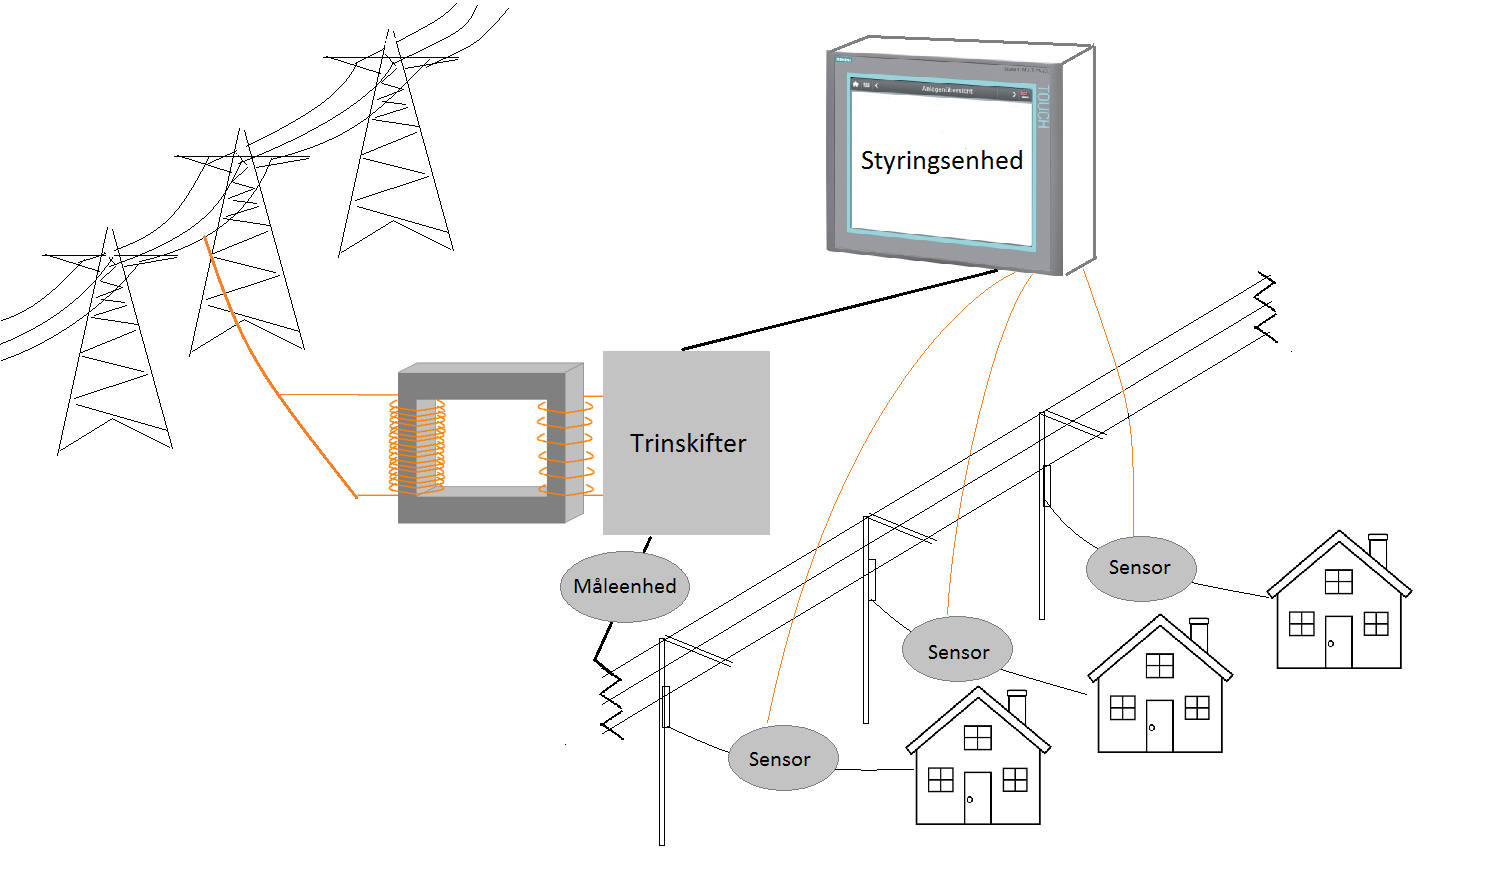
\includegraphics[width=1\textwidth]{figure/RigtBillede}
	\caption{Visuel fremstilling af Spændingsregulator}
	\label{fig:Rigtbillede}
\end{figure}

På figur \ref{fig:Rigtbillede} ses en illustration, der giver oveblik over Spændingsregulatoren. Billedet viser trintransformeren, der forsyner distributionslinjen, sensorer, der måler aktuelle værdier på linjen og en styringsenhed, der regulerer trintransformeren på baggrund af disse værdier. 
% !TEX root = ../prj4projektrapport.tex
% SKAL STÅ I TOPPEN AF ALLE FILER FOR AT MASTER-filen KOMPILERES 

Dette kapitel indeholder en overordnet beskrivelse af systemet, samt en gennemgang af de funktionelle og ikke funktionelle krav der stilles til systemet. 

\section{Systembeskrivelse}
Spændingsregulatoren skal være i stand til at analysere forholdene på distributionslinjen. Derfor udvikles en måleenhed, som kan placeres decentralt, ved hver forbruger, og centralt ved spændingsregulatoren. Måleenhederne skal sende værdier for spænding, strøm, powerfactor og indhold af harmoniske til et system, som regulerer spændingen på baggrund af disse målinger. 

Spændingsreguleringen laves med en trintransformer, hvor der med en styringsenhed kan skiftes mellem trinene. Styringsenheden kan automatisk regulere spændingen jf. data fra måleenhederne, eller den kan styres manuelt på en grafisk brugergrænseflade. 

Systemet der er udviklet i dette projekt er proof of concept, så spændingsniveauet er skalleret ned.  Der er designet et simuleringskredsløb i form af en distributionslinje og en række forbrugere, for at vise funktionaliteten af Spændingsregulatoren. Forbrugerene  kan kobles til/fra nettet, for at generere et spændingsfald der giver anledning til en regulering af trintransformeren. 


% !TEX root = ../../prj4projektrapport.tex
% SKAL STÅ I TOPPEN AF ALLE FILER FOR AT MASTER-filen KOMPILERES 

\section{Foranalyse for Styringsenhed}

\subsection{Kontrolmodul og Brugergrænseflade}
Det er en oplagt mulighed at anvende en PLC og et HMI, som Kontrolmodul og Brugergrænseflade i projektet. Dette skyldes at der, som krav til projektet skulle anvendes relevante faglige elementer fra semestrets kurser. Faget Instrumentering og Automatisering(IOA) omhandler netop brugen af PLC og HMI i industrien. Hermed kommer to gode argumenter for PLC og HMI; relevant faglige viden anvendes og i den virkelige verden ville det være oplagt at bruge lignende enheder til et projekt som dette.


PLC'en kan programmeres i flere forskellig sprog. Ladder er dog blevet valgt, fordi det er det mest anvendte i IOA. Desuden er det et krav til projektet at en bruger skal kunne interagere med systemet, hvilket opnåes gennem HMI'et.


Kravet om pålidelig transmission af data mellem udvalgte enheder understøtter også valget af en PLC, da denne indeholder mulighed for LAN kommunikation gennem en RJ-45 port.

\subsection{Kommunikationsmodul}
Det blev hurtigt i projektfasen valgt at der skulle udvikles kommunikation over en LAN forbindelse, da det i projektet var et krav at der skal være pålidelig transmission af data mellem udvalgte enheder. Der blev undersøgt hvilke muligheder der var for at gøre kommunikation over en LAN forbindelse med en microcontroller muligt, da vi allerede havde haft PSoC og Arduino programmering blev der i Embedded Stock bestilt et ethernet shield til hver af disse. Men da Måleenheden bliver implementeret på en PSoC blev det besluttet at prøve at implementere LAN kommunikationen på samme PSoC, som en af Måleenhederne. 


Arduinoen blev holdt som en back-up mulighed, da det er et lettere udviklingsmiljø og samtidig mere populært end PSoC-miljøet, hvorfor der også er mere hjælp at finde om Arduinoen på nettet. Det ville dog være nødvendigt at anvende en anden form for kommunikation mellem Måleenhederne og Arduinoen. 





%Krav: Systemet skal omfatte pålidelig transmission af data mellem udvalgte enheder.
%Komunikationsmodul + shields
%Kommunikationsformer
%Arduino udviklingsmiljø


% !TEX root = ../../prj4projektdokumentation.tex
% SKAL STÅ I TOPPEN AF ALLE FILER FOR AT MASTER-filen KOMPILERES 

\chapter{Arkitektur}

\include{sektioner/DesignOgImplementering}
\include{sektioner/ResultatOgDiskussion}
\include{sektioner/FremtidigtArbejde}
% !TEX root = ../prj4projektrapport.tex
% SKAL STÅ I TOPPEN AF ALLE FILER FOR AT MASTER-filen KOMPILERES 


Projektets formål har været at undersøge, hvordan spændingen kan holdes stabil i et system med varierende belastninger. Dette blev løst ved at udvikle en Spændingsregulator, der kan skifte spændingsniveauer på en trintransformer og derved sikre en bestemt spænding hos forbrugerne, selv om forbruget ændres. Dette har dog vist sig ikke at være relevant i det danske distributionssystem, men projektets overordnede proof of concept er gennemført. Det er implementeret, at Spændingsregulatoren kan observere THD i systemet. Dette har dog også vist sig ikke at være brugbart på distributionsnettet. Det kan derfor konkluderes, at det på nuværende tidspunkt ikke er relevant at implementere i det danske elnet, men at det i fremtiden måske kan blive en del af en smart grid løsning. Projektgruppen har dog løst problemformuleringen og opfyldt kravene til projektet. Gruppen er desuden stolte af, at have fået systemet til at fungere automatisk, selvom det var nedprioriteret i MoSCoW'en. Gennem projektforløbet har gruppen fået kendskab til problematikker og udfordringer i det danske elnet samt fået erfaringer inden for kommunikationsprotokoller, PLC programmering og påvirkning fra harmoniske.  


Der er lavet et grundigt forarbejde og en fornuftigt arbejdsfordeling, hvilket har medført, at tidsplanen er overholdt og et tilfredsstillende resultat er opnået. Opgaver i forbindelse med udviklingen af Spændingsregulatoren har været uddelt i tre hold. Der har været god kommunikation holdene imellem, hvilket har givet en forholdsvis nem integrationsfase uden de store udfordringer. Samlet set har gruppen fået et godt udbytte af projektet både fagligt og inden for projektstyring.



 
\include{sektioner/Udviklingsvaerktoejer}
% !TEX root = ../prj4projektrapport.tex
% SKAL STÅ I TOPPEN AF ALLE FILER FOR AT MASTER-filen KOMPILERES 
%%%%%%%%%%%%%%%%%%%%%%%
\mainmatter



\printbibliography

\end{document}


